\chapter{Kalibrace kamery}
Kalibrace kamery znamená nalezení jejich vnitřních a vnějších parametrů.
Má využití v počítačovém vidění, pro skládání obrazu z více snímků nebo pro vytváření 3D modelů.


Kalibrace kamery se dá provádět s nebo bez pomoci snímků, na nichž se nachází známé kalibrační objekty.
V této kapitole se zaměříme na srovnání dvou odlišných metod kalibrace kamery, které nevyžadují kalibrační objekty, a to na \cite{Lalonde10} a \cite{deepcalib}.


\section{Kalibrace kamery pomocí optimalizace nad snímky z meteorologických webových kamer}
Tuto metodu představil \cite{Lalonde10}. 
Předpokládá, že kamera je namířena na oblohu a že se v průběru času nemění její pozice ani orientace. 
Dále předpokládá, že kamera je umístěná vodorovně – tedy že horizont je na snímku rovnoběžný se spodní hranou snímku.
Vyžaduje z každé kamery několik snímků v průběhu několika dní v rýzných denních hodinách.

Je založená na optimalizaci čtverce rozdílu obrazu skutečné oblohy a oblohy vygenerované modelem oblohy. 
K nalezení optimálních parametrů modelu oblohy využívá nelineární metodu nejmenších čtverců (non-linear least squares).
Algoritmus dokáže určit zenit $\theta_c$, azimut $\phi_c$ a ohniskovou vzdálenost $f_c$.
Program vyžaduje, aby byla k dispozici sémantická segmentace oblohy, aby optimalizace nesrovnávala krajinu s modelem oblohy. Perez tuto segmentaci prováděl ručně. 
K určení $f_c$ a $\theta_c$ využívá dataset $\mathcal{I}$ a k určení $\phi_c$ využívá dataset $\mathcal{J}_c$. 


\paragraph{Značení}
\begin{itemize}
    \item $\mathcal{D}_c$ – množina snímků oblohy kamerou $c$ s neznámými parametry ($\theta_c, \phi_c, f$)
    \item $y^{(i)}_p$ – jas na pozici $(u_p, v_p)$ v obrázku $i$
    \item $\mathcal{P}_c  = \{p | segmentace(y_{p}) = obloha\}$ – pixely označení sémantickou segmentací jako obloha
    \item $v_{min} = min\{ v_p | p \in \mathcal{P}_c \}$ – pozice na ose $y$ nejníže položeného pixelu oblohy
    \item $\theta^{(j)}_s, \phi^{(j)}_s$ – zenit a azimut slunce v čase pořízení snímku $j$
\end{itemize}

\subsection{Tvorba datasetu $\mathcal{I}_c$ a $\mathcal{J}_c$}

\paragraph{Množina $\mathcal{I}_c$}


Chceme najít množinu $\mathcal{I}_c \subseteq \mathcal{D}_c$, která obsahuje snímky čisté oblohy bez oblačnosti, se sluncem co nejdále od zorného pole kamery.

Toho docílíme aproximací každého snímku oblohy pomocí
\begin{equation}
    \hat{y}^{(i)}_{p} = \alpha_i(v_p - v_{min})^2 + \beta_i,
\end{equation}

Parametry $\alpha_i$ a $\beta_i$ určíme metodou nejmenších čtverců:
\begin{lemma}[Nalezení ($\alpha_i, \beta_i$) metodou nejmenších čtverců]
Nechť $P = |\mathcal{P}_c|$
$$A = \begin{bmatrix} (v_1 - v_{min})^2 & 1 \\ \vdots & \vdots \\ (v_P - v_{min})^2 & 1\end{bmatrix}, b = \begin{pmatrix} y_1 \\ \vdots \\ y_P \end{pmatrix}.$$
Pak $x = \T{( \alpha_i,  \beta_i )} = (A^\top A)^{-1} A^\top b$.
\end{lemma}

Abychom vytvořili $\mathcal{I}_c$, vezmeme snímky s $\alpha_i < 0$, poté z nich vybereme 10~\% s nejnižším reziduem $||Ax-b||$ a potom vezmeme $N$ s nejnižší |$\alpha_i$|.

\paragraph{Množina $\mathcal{J}_c$}
Dataset $\mathcal{J}_c \subseteq \mathcal{D}_c$ sloužící k nalezení zenitu $\phi_c$ obsahuje snímky jasné oblohy, kde jsou patrné známky toho, že slunce je blízko zorného pole kamery.
Není však žádoucí, aby slunce bylo přímo na snímku, protože pak by ve snímku nastaly problémy s expozicí a šumem.
Lalonde navrhl $\mathcal{J}_c$ vytvořit tak, že vybere 4 dny s nejvyšším počtem snímků s $\alpha < 0$. Tím by měl získat slunečné dny. 
Poté ze snímků pořizovaných v průběhu celého dne vybere $N$ snímků s nejmenším vertikálním a horizontálním gradientem, na kterých by měla být nejčistší obloha.

\begin{figure}[htb]\centering
    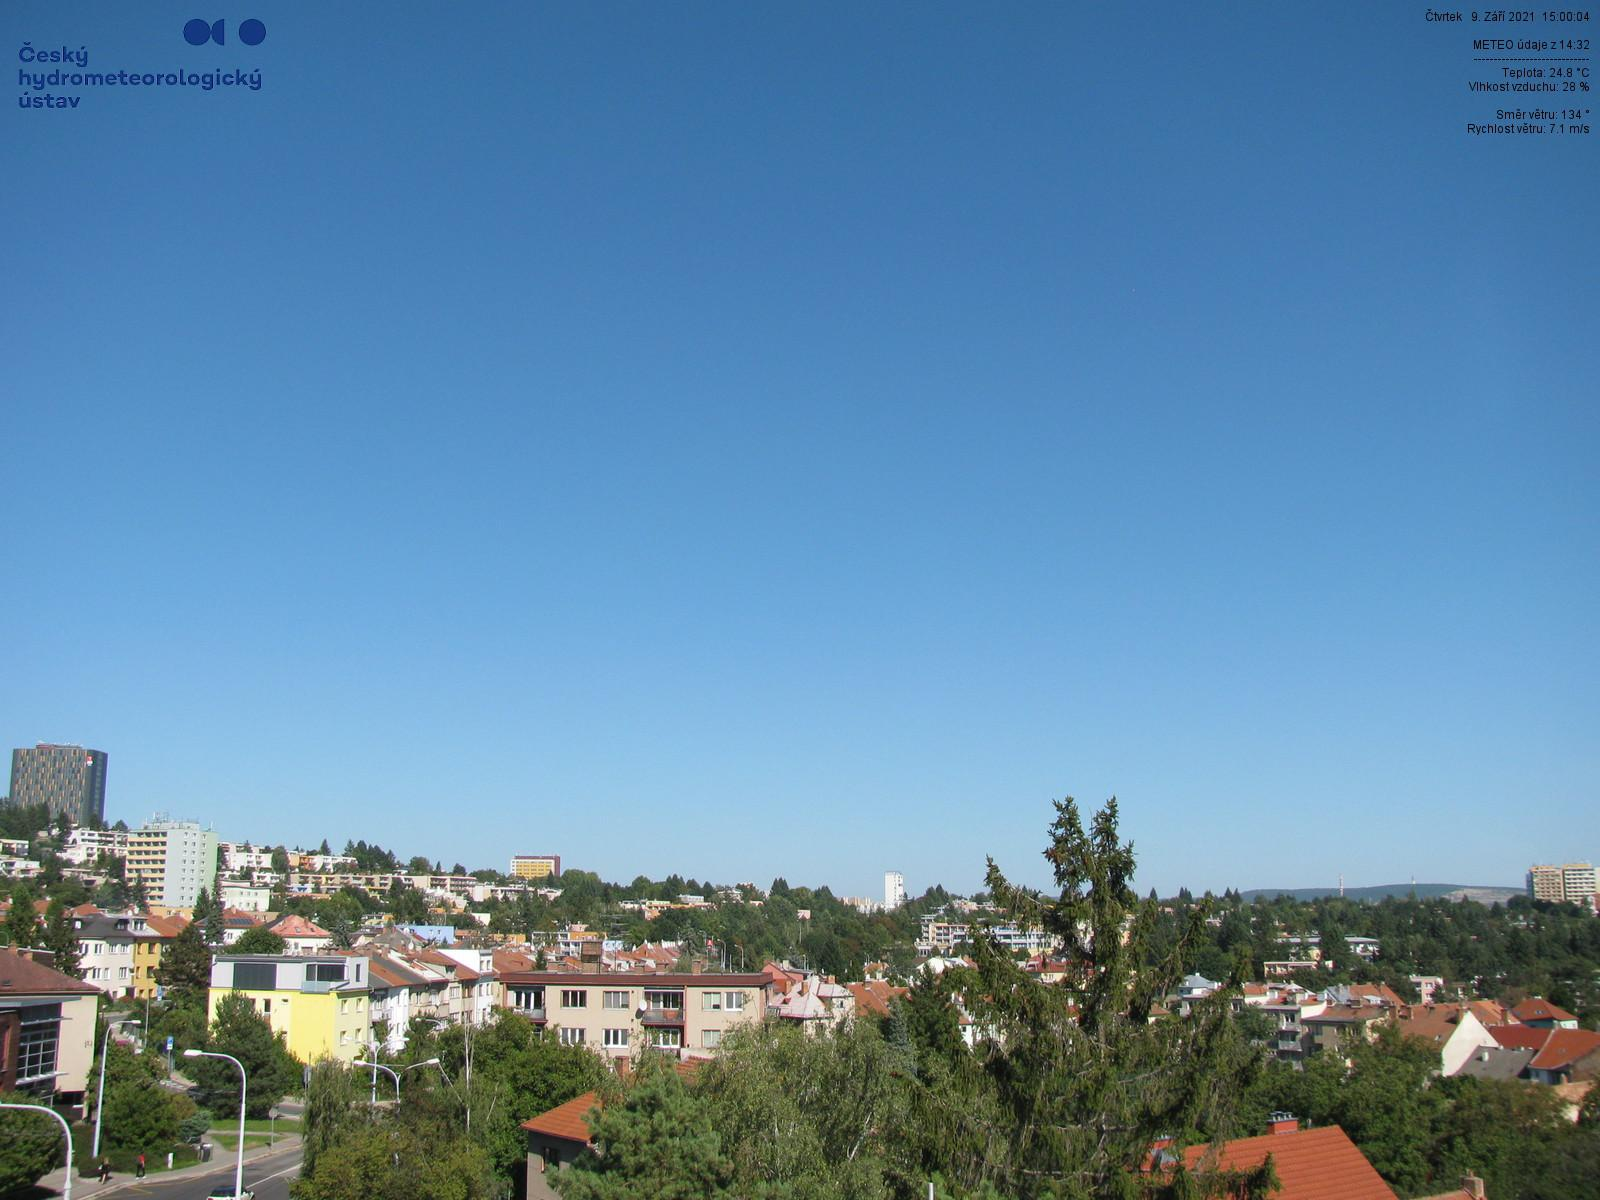
\includegraphics[width=100mm]{../img/horizontalgradient}
    \caption{Příklad snímku z datasetu $\mathcal{I}_c$ \citep{chmu}}
\end{figure}

\begin{figure}[htb]\centering
    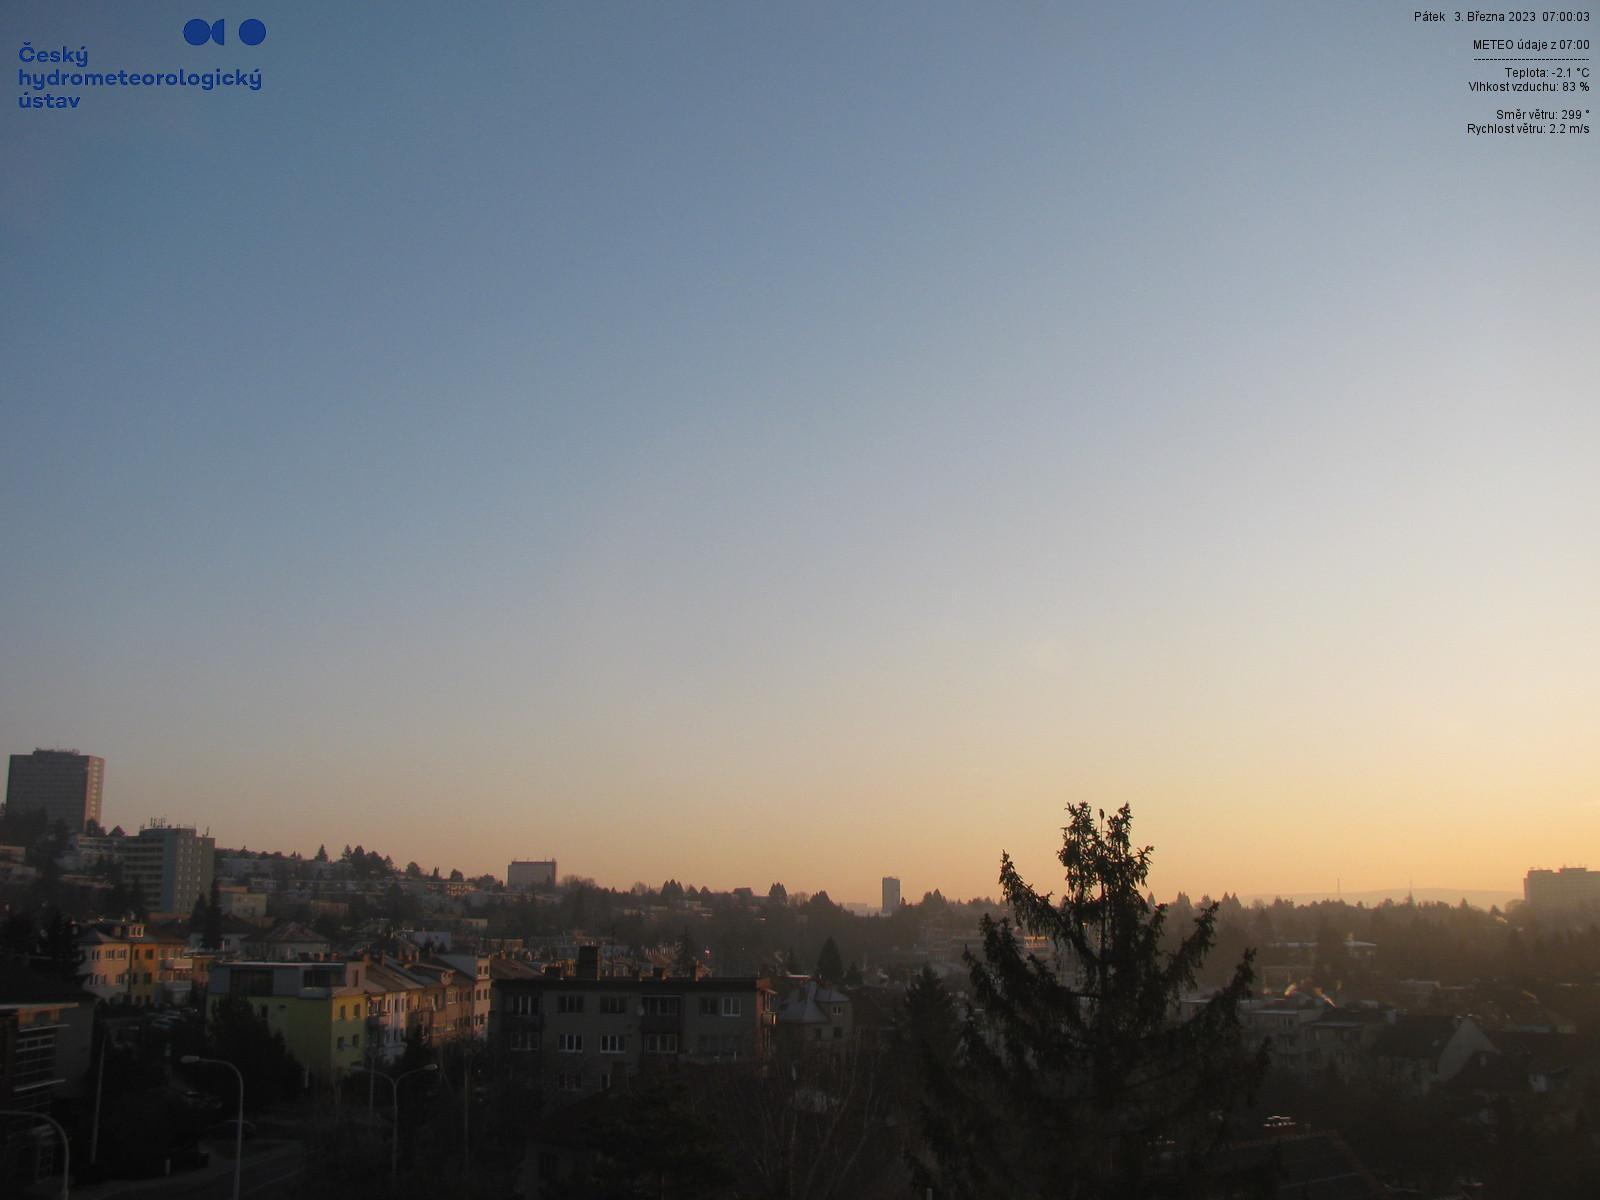
\includegraphics[width=100mm]{../img/sungradient}
    \caption{Příklad snímku z datasetu $\mathcal{J}_c$ \citep{chmu}}
\end{figure}

\subsection{Optimalizace}

Hledané parametry $\theta_c, \phi_c, f_c$ najdeme nelineární metodou nejmenších čtverců algoritmem LM (Levenberg-Marquardt) \citep{levenberg}.


\begin{equation}
    \hat{f_c}, \hat{\theta_c}, \hat{k}^{(i)} = \arg\min_{\theta_c, f_c, k^{(i)}}  \sum_{i\in\mathcal{I}_c} \sum_{p\in\mathcal{P}_c} \left( y^{(i)}_p - k^{(i)}g'(u_p, v_p, \theta_c, f_c)\right)^2
\end{equation}

\begin{equation}
    \hat{\phi_c}, \hat{k}^{(j)} = \arg\min_{\phi_c, k^{(j)}}  \sum_{j\in\mathcal{J}_c} \sum_{p\in\mathcal{P}_c} \left( y^{(j)}_p - k^{(j)}g(u_p, v_p, \hat{\theta_c}, \phi_c, \hat{f_c}, \theta^{(j)}_s, \phi^{(j)}_s)\right)^2
\end{equation}


    




\section{Kalibrace kamery pomocí hlubokých neuronových sítí}
Práce \cite{deepcalib} představuje metodu, jak z jediného snímku určit její příčný náklon $\psi_c$, zenit $\theta_c$, ohniskovou vzdálenost $f_c$ a zkreslení čočky $\xi_c$.
Oproti předchozí metodě má méně specifický vstup a proto i širší použití. 
Nevyužívá však znalost o pozici slunce v době pořízení snímku, takže nemá jak určit azimut kamery $\phi_c$.
Spíše než k tvorbě datových podkladů pro trénování neuronových sítí tedy může sloužit ke vkládání 3D objektů do snímků nebo nápravě zkreslení čočky.

Metoda staví na konvoluční neuronové síti s architekturou DenseNet \citeauthor{densenet} předtrénované na obrazové databázi ImageNet \citep{imagenet}. 
Výstupní vrstva tohoto modelu je potom nahrazena čtyřmi výstupy: náklon $\psi$, vzdálenost horizontu od středu obrázku $v_m$, zorný úhel $h_\theta$, a zakřivení $\xi$.
Síť je dotrénována na datasetu 360Cities \citep{360cities}. Trénování probíhá pomocí algoritmu Adam \citep{adam} s využitím ztrátové funkce KL divergence \citep{kldivergence}.

\begin{figure}[htb]\centering
    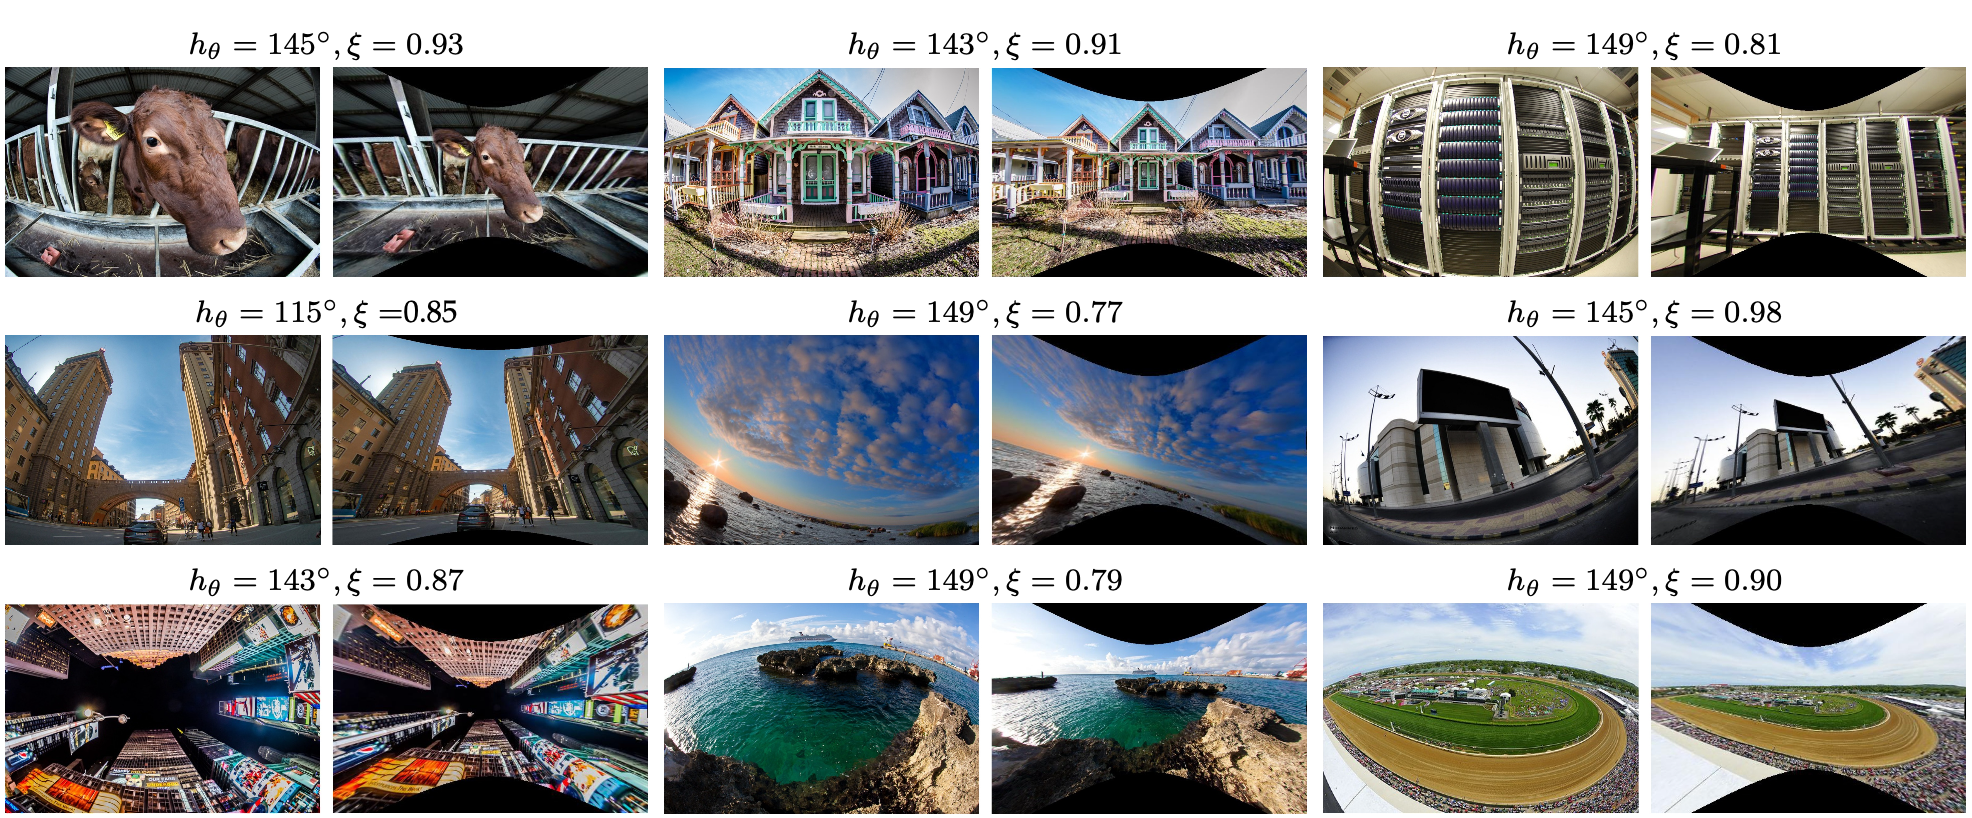
\includegraphics[width=140mm]{../img/distortion}
    \caption{Automatická oprava zkreslení čočky \citep{deepcalib}}
\end{figure}

\begin{figure}[htb]\centering
    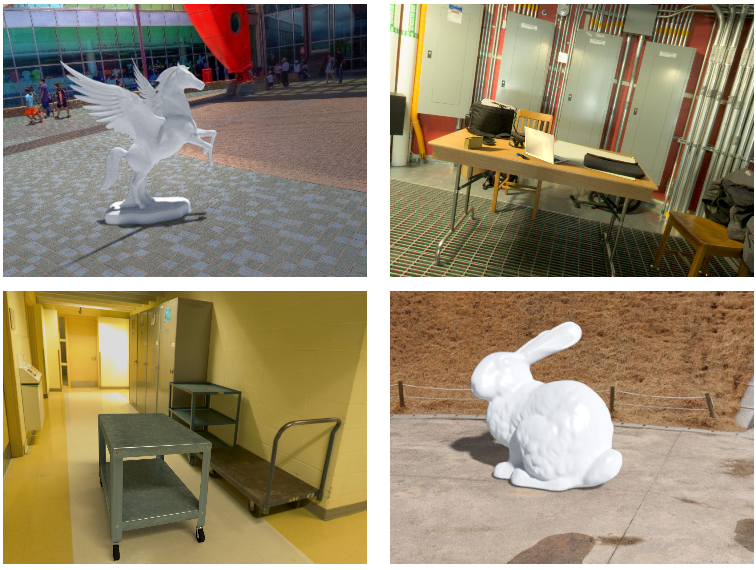
\includegraphics[width=100mm]{../img/3d}
    \caption{Realistické vkládání 3D objektů do snímků \citep{deepcalib}}
\end{figure}





\chapter{Data}
Práce využívá obrazových dat z veřejně dostupných webových meteorologických kamer Českého hydrometeorologického ústavu (ČHMÚ).
\begin{figure}[h]\centering
    \includegraphics[width=140mm]{../img/map}
    \caption{Mapa webových kamer \cite{chmu}}

\end{figure}